\chapter{File Protection}
	\section{Built in protection}
	It's important to know that usually, operating systems do not have a built in mechanism that include a password protection method. However, there is a file permission policy that counts as a level of protection from other users.
	
	\subsection{Windows}
	File protection in Windows can be achieved through DACLs (discretionary access control lists). As a short explanation, a Windows object can have a DACL which contains ACEs(access control entries) that define what type of access any user or group of users can have. \cite{MDSNDACsLACEs}
		
	Usually, DACLs are used by defining the users and groups that can have access because the ones that are not included will have restricted access by default. If a DACL does not contain any ACEs the system will deny any type of access.
	
	\begin{figure}[h!]
		\includegraphics[width=\linewidth]{images/securitySettings.jpg}
		\caption{Advanced Security Settings dialog}
		\label{fig:securitySettings}
	\end{figure}
	
	Let us consider a new text file named "demo file.txt" on a Windows 10 OS that has 2 users, namely user" and user 1, which both have administrator permissions. To restrict access for user1 I have to go to file's properties \textbf{Security}-\textgreater\textbf{Advanced}.

	In figure \ref{fig:securitySettings} we can see the "Permission Entries" which maps to DACL we mentioned earlier whilst list's entries map to ACEs. I added the Administrators and user to have full control, and also I set user 1's permissions to deny any type of action. In this example we can notice that order in which permissions are set matters because user 1 cannot access the file, even if that user takes part from Administrator's group. 
	
	At the moment only the current user and other possible users in the Administrator group could have access to the file. Still, we are not fully protected when it comes for example to exploits. We could consider that we are logged in with user 1, which currently does not have any kind of permission for the demo file. There is the possibility of an exploit having first user's permissions and overwriting, encrypting or deleting the file which would be disastrous.
	
	
	\subsection{Linux}
	Almost the same mechanism exists in Linux, but it's more trivial. In my examples I will talk about Ubuntu, but the mechanism is almost the same for most of the Linux distributions.
		
	\section{Existing products for Windows}
	As a similar tool, a first one that draws attention, is iBoysoft's File Protector for Windows, coming as a 7-day free trial or a payed version. As a main functionality, this tool allows the user to select the desired folders or files to be protected, along with the protection type (i.e. read/write/delete).
	
	The application starts with a message box, demanding a password. After it was inserted correctly, the application starts, displaying on the main screen a list of files and folders the user has chosen to be protected.
	
	\begin{figure}[h!]
		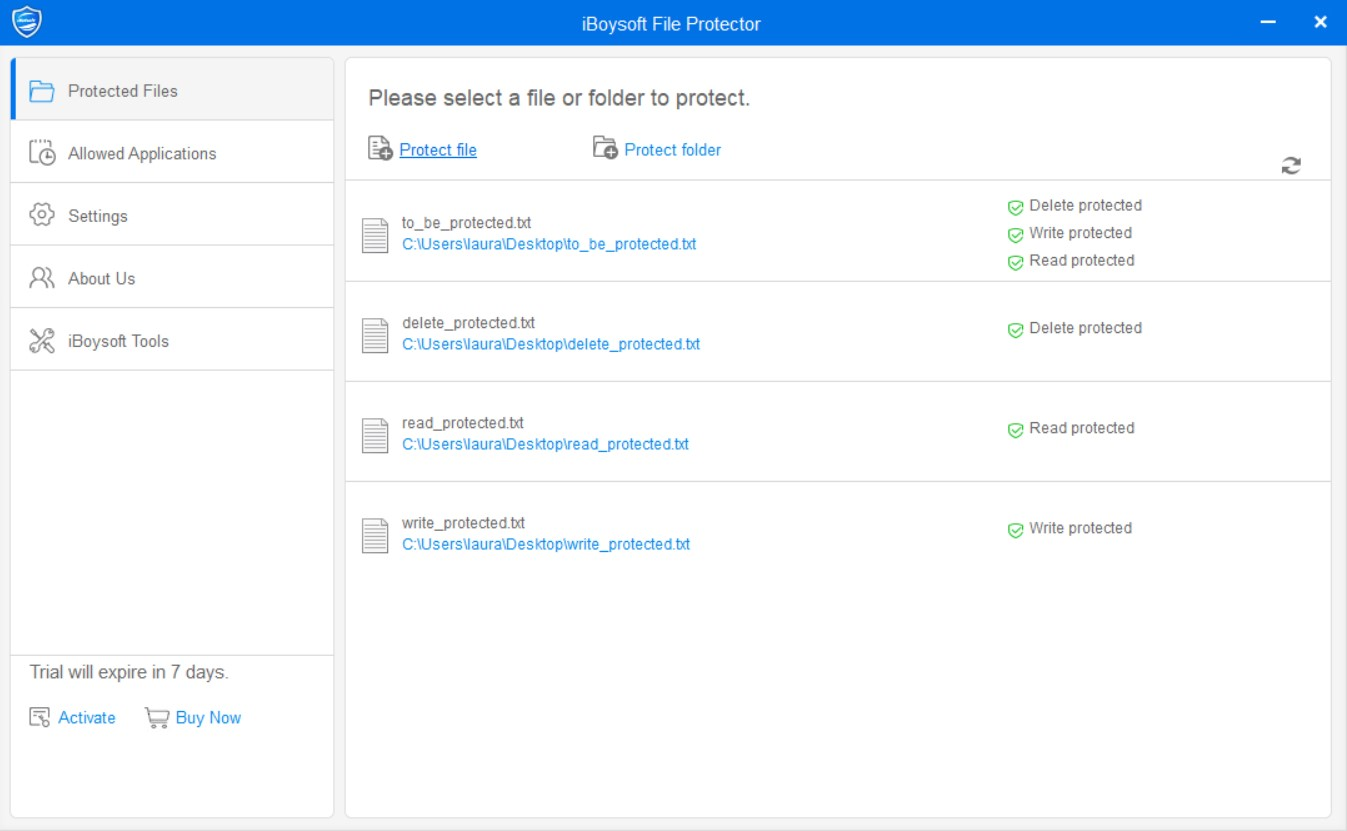
\includegraphics[width=\linewidth]{images/iBoysoftMain.jpg}
		\caption{iBoysoft File Protector for Windows}
		\label{fig:iBoysoftFP}
	\end{figure}
	
	In figure \ref{fig:iBoysoftFP} we can see the main screen of the application, where we have a list of protected files, buttons for adding files or folders, and also the menu on the right. 
	
	Another feature of this tool is the allowed applications. There, the user can choose which applications that can have rights, in spite of the protection selected for the file or folder. After adding an application, the user should also add the files or folders that application can have access to.
	
	If for example a text file was added to the list with read protection, that file cannot be opened by the user, which is a drawback for this application. There is one thing that can be done, and that is giving permissions to other applications to perform actions upon the desired files.
	
	There is also the settings tab which contains two important sections, one where you can change the password, another one where you can choose the default protection types that are selected when adding a file or folder.
	
	As a conclusion, the only time a password is required, is when the application is started. 
	
	*find another soft like this
	
	\newpage
	\section{Used Technologies}
		There are three main technologies that I want to talk about in the next subsections, namely Windows Filter Manager, which is important as a concept to be understood, C and .NET where I will explain my choice. //TODO
		\subsection{Windows Filter Manager}
		
		
		concepts : Altitude
		
			
		
	\newpage
	\section{Design and Implementation}
		\subsection{Minifilter High Level Overview of Design}
		//TODO
		* describe the structure of the minifilter driver
		
		\subsection{IRP Filtering}
		IRPs (I/O request packets) are Windows kernel mode structures that are used to incorporate . 
		
		* what type of IRPs exist
		
		* which IRPs I filter
		
		* how i filter the IRPs 
		
		\subsection{Monitoring and Denying Access}
		//TODO
		
		*diagram + code of how and where exactly it happens
		
		\subsection{Encountered Challenges}
		//TODO  
		
		* process of installation of a minifilter driver on a test machine
		
		\subsection{Inter Component Communication}
		//TODO
		
		* make some diagrams to make it more clear
		
		
	\newpage
	
	\section{Testing Approach}
		In order to achieve a reliable software, the application has been tested using both black box and white box testing methods, which will be described in the following sections.
		
		\subsection{Driver Verifier}
		First of all I will describe some basic functionalities of Driver Verifier, that I have also used to test the minifilter.
		
		As the name suggests, Driver Verifier is a tool that can monitor Windows kernel drivers. It can detect major problems, such as memory leaks, memory corruptions or deadlocks. This tool is developed by Microsoft, making it's first appearance in Windows XP as a command line utility. Over the time this tool has gained more checks as well as a graphical user interface namely Driver Verifier Manager, that allow a programmer to select the preferences for driver's testing.
		
		\subsection{Static Code Analysis}
		In this section I will talk about source code annotation language (SAL). This is used to make the code more explicit, in terms of behavior, parameters, return values, or other things* to make it more understandable. In other words, programmer's work is to use annotations considering the desired functionalities, and compiler's work is to verify if the written code corresponds with the annotations. 
		
		Another benefit of SAL is that specifications in the form of code comments and documentation are validated by the annotations. This is an advantage because in some cases the documentation or comments can be vague, making it hard for a programmer to integrate the code correctly. Moreover, if SAL is used, the compiler can validate that the code written meets the documentation and specifications.
		
		All SAL annotations have a specific "look", and that is \texttt{\_Annotation\_name\_}. For example, some parameter most used SAL annotations are \texttt{\_In\_} and \texttt{\_Out\_}. \texttt{\_In\_} makes sure the compiler interprets data as being input data that cannot be modified in function's scope. \texttt{\_Out\_} allows the programmer to use the parameter as an output one, as long as the space for that parameter has been allocated by the programmer.
		
		As for behavior, a simple example is \texttt{\_Check\_return\_}. If this annotation is used, the caller must inspect the returned value. In case the function has a void return type, an error will be shown at compilation time. A similar example is \texttt{\_Must\_inspect\_result\_}, which contains the functionality of \texttt{\_Check\_return\_} and adds that any output parameter should also be used after the function call.
		
		After these examples anyone should be convinced that SAL is beneficial from multiple reasons, and that is also why I used it in my own code.
		
		//TODO
		My code examples
		